\documentclass[11pt,table,final,fleqn,xcolor={usenames,dvipsnames},handout]{beamer}
\usetheme[]{Frankfurt}
\usecolortheme{crane}

% \usepackage{listings}
% \usepackage{multimedia} % Movies
% \usepackage{fancyvrb,relsize}
% \usepackage{commath}
% \usepackage{graphicx}
% \usepackage{longtable}
% \usepackage[math]{iwona}
% \usepackage{wasysym}
% \usepackage{amsmath}
% \usepackage{amssymb}
% \usepackage[amssymb]{SIunits}
% \usepackage{tikz} % Drawing


\usepackage{listings}
\usepackage{multimedia} % Movies
\usepackage{fancyvrb,relsize}
\usepackage{commath}
\usepackage{graphicx}
\usepackage{array}
\usepackage{longtable}
\usepackage{algpseudocode} 
\usepackage{multirow}
\usepackage[math]{iwona}
\usepackage{wasysym}
% \usepackage[fleqn]{amsmath}
\usepackage{amssymb}
\usepackage{siunitx}
\usepackage{tikz} % Drawing
\usepackage{pgfplots}
\usepackage{pgfplotstable}
% \usepackage{fontspec}

% Presentation settings
\rowcolors[]{1}{maincolor!20}{maincolor!10}

\newcommand{\Fo}{\ensuremath{\mathit{Fo}}}

\lstset{language=Matlab,%
    %basicstyle=\color{red},
    basicstyle=\scriptsize\ttfamily,
    breaklines=true,%
    morekeywords={matlab2tikz},
    keywordstyle=\color{blue},%
    morekeywords=[2]{1}, keywordstyle=[2]{\color{black}},
    identifierstyle=\color{black},%
    stringstyle=\color{mylilas},
    commentstyle=\color{mygreen},%
    showstringspaces=false,%without this there will be a symbol in the places where there is a space
    numbers=none,%
%     numberstyle={\tiny \color{black}},% size of the numbers
%     numbersep=-2pt, % this defines how far the numbers are from the text
%     emph=[1]{for,end,break},emphstyle=[1]\color{red}, %some words to emphasise
emph=[2]{ones,int,str2double,long,single,simplify,diff,log,atan,solve,vpa,syms,doc,int,simplify,diff,log,atan,syms,interp3,interpn,histogram,ribbon,contourf,fzero,feval,fminsearch,fsolve,fminbnd,ezplot,varargin,optimset,odeset,ode15s,plotyy,ones,linprog,cftool,optimset,lsqnonlin}, emphstyle=[2]{\color{blue}},
    backgroundcolor=\color{gray!15},frame=tlbr, framerule=0pt,
    escapeinside={(*@}{@*)}
}

% To have the navigation circles without declaring subsections
\usepackage{remreset}% tiny package containing just the \@removefromreset command
\makeatletter
\@removefromreset{subsection}{section}
\makeatother
\setcounter{subsection}{1}

% For convenient figure inclusion
\DeclareGraphicsExtensions{.pdf,.png,.jpg}
\graphicspath{ {../img/} }


% \setmainfont{Yanone Kaffeesatz}
% \setmathfont(Digits,Latin,Greek)[Numbers={Lining,Proportional}]{Gentium Plus}

% TU/e colors
\definecolor{tuered}{RGB}{247,49,49}
\definecolor{tuefuchsia}{RGB}{214,0,74}
\definecolor{tuelila}{RGB}{214,0,123}
\definecolor{tuepurple}{RGB}{173,32,173}
\definecolor{tuedblue}{RGB}{16,16,115}
\definecolor{tueblue}{RGB}{0,102,204}
\definecolor{tuelblue}{RGB}{0,162,222}
\definecolor{tueorange}{RGB}{255,154,0}
\definecolor{tueyellow}{RGB}{255,221,0}
\definecolor{tuedyellow}{RGB}{206,223,0}
\definecolor{tuegreen}{RGB}{132,210,0}
\definecolor{tuedgreen}{RGB}{0,172,130}
\definecolor{tueblue2}{RGB}{0,146,181}

% For Matlab script colors
\definecolor{mygreen}{RGB}{28,172,0} % color values Red, Green, Blue
\definecolor{mylilas}{RGB}{170,55,241}

\makeatletter
% \definecolor{beamer@blendedblue}{rgb}{0.5,0.5,0.3} % changed this
\useoutertheme{smoothbars}
\useinnertheme{circles}

%%%%%%%%%%%%%%%%%%%%%%%%%%%%%%%%%%%%%%%%%%%%%%%%%%%%%%%%%%%%%%%%%%%%%%%%%%%
\definecolor{maincolor}{named}{tuelblue}
\definecolor{textcolorfg}{named}{white}
\definecolor{tuealert}{named}{tueblue}
%%%%%%%%%%%%%%%%%%%%%%%%%%%%%%%%%%%%%%%%%%%%%%%%%%%%%%%%%%%%%%%%%%%%%%%%%%%

\setbeamercolor{normal text}{fg=black,bg=white}
\setbeamercolor{alerted text}{fg=tuealert}
\setbeamercolor{example text}{fg=tuegreen!50!black}

\setbeamercolor{background canvas}{parent=normal text,bg=white}
\setbeamercolor{background}{parent=background canvas}

\setbeamercolor{title}{bg=maincolor,fg=textcolorfg} % Presentation title colors
\setbeamercolor{structure}{fg=maincolor,bg=textcolorfg}
\setbeamercolor{section in head/foot}{fg=textcolorfg,bg=maincolor}
\setbeamercolor{palette primary}{fg=textcolorfg,bg=maincolor} % changed this

\setbeamercolor{palette primary}{fg=maincolor,bg=textcolorfg} % changed this
\setbeamercolor{palette secondary}{use=structure,fg=structure.fg!100!tueblue} % changed this
\setbeamercolor{palette tertiary}{use=structure,fg=structure.fg!100!tuered} % changed this

\setbeamertemplate{navigation symbols}{} % ( Dont use )
\setbeamercolor{navigation symbols}{use=structure,fg=structure.fg!40!bg}
\setbeamercolor{navigation symbols dimmed}{use=structure,fg=structure.fg!20!bg}

\setbeamercolor{block title}{fg=textcolorfg,bg=maincolor}
\setbeamercolor{block body}{fg=black,bg=maincolor!10}

\def\colorize<#1>{%
  \temporal<#1>{\color{tuedblue!40!gray!40}}{\color{tuealert}}{\color{black}}}
  
\setlength{\mathindent}{0pt}

\makeatother

% Colored urls
\hypersetup{colorlinks,linkcolor=,urlcolor=tueblue}

% Vector format
\renewcommand{\vec}[1]{\mathbf{#1}}

\usetikzlibrary{decorations} % Drawing
\usetikzlibrary{patterns}
\usetikzlibrary{positioning}
\usetikzlibrary{shadows}
\usetikzlibrary{calc}
\usetikzlibrary{arrows}
\usetikzlibrary{decorations}
\usetikzlibrary{plotmarks}
\usetikzlibrary{shapes}
\usetikzlibrary{shadings}
\usetikzlibrary{intersections}
% Blocks
\tikzset{block/.style={rectangle,draw=maincolor,fill=maincolor!20,text width=10em,text centered,rounded corners,minimum height=4em,thick}}
\tikzset{emphblock/.style={rectangle,draw=maincolor,text centered,rounded corners,thick,top color=maincolor!10,bottom color=maincolor!30}}
% Dots
\tikzset{dot/.style={draw=tuered,circle,thick,minimum size=1mm,inner sep=0pt,outer sep=0pt,fill=white}}
\tikzset{fdot/.style={circle,draw=black,fill=black,,inner sep=1.5pt}}
\tikzset{gdot/.style={circle,draw=black,inner sep=3pt}}
\tikzset{cross/.style={cross out, draw=black, fill=none, minimum size=2*(#1-\pgflinewidth), inner sep=0pt, outer sep=0pt}, cross/.default={4pt}}
% Graphs and lines
\tikzset{line/.style={black,>=stealth',semithick}}
\tikzset{graph/.style={smooth,samples=400,tuered,semithick}}
\tikzset{interp/.style={dot,draw=tuealert,inner sep=1.5pt,minimum size=4pt,color=tuealert,fill=none}}
\tikzset{intblock/.style={line,draw=tuefuchsia,fill=tuefuchsia!50!white,fill opacity=0.3,opacity=0.6}}
\tikzset{intdot/.style={line,dot,draw=tuefuchsia,fill=tuefuchsia,opacity=0.6}}
\tikzset{gridline/.style={lightgray,ultra thin,dashed}}


\newcolumntype{L}[1]{>{\raggedright\arraybackslash}p{#1}}
\newcolumntype{R}[1]{>{\raggedleft\arraybackslash}p{#1}}

% \pgfplotsset{
% % every axis y label/.append style={at={axis cs:14,14},rotate=0,anchor=south east}
% exery axis/.style={ylabel near ticks},
% }


\renewcommand*\familydefault{\sfdefault}  % Use sans font
% 
% \usepackage{pgfpages}
% \pgfpagesuselayout{4 on 1}[border shrink=5mm]

% PRESENTATION SPECIFICS
\title{Numerical Methods for Chemical Engineers}
\subtitle{Study guide for 6E5X0, 2016-2017}

\author[I.~Roghair]{\underline{Ivo~Roghair}, Martin van Sint Annaland}

\institute{Chemical Process Intensification\\Eindhoven University of Technology}

\date{13 November 2017}

% BEGIN PRESENTATION
\begin{document}
\lstset{language=Matlab,%
    %basicstyle=\color{red},
    basicstyle=\footnotesize\ttfamily,
    breaklines=true,%
    morekeywords={matlab2tikz},
    keywordstyle=\color{blue},%
    morekeywords=[2]{1}, keywordstyle=[2]{\color{black}},
    identifierstyle=\color{black},%
    stringstyle=\color{mylilas},
    commentstyle=\color{mygreen},%
    showstringspaces=false,%without this there will be a symbol in the places where there is a space
    numbers=none,%
%     numberstyle={\tiny \color{black}},% size of the numbers
%     numbersep=-2pt, % this defines how far the numbers are from the text
%     emph=[1]{for,end,break},emphstyle=[1]\color{red}, %some words to emphasise
    emph=[2]{int,simplify,diff,log,atan,syms}, emphstyle=[2]{\color{blue}}
}

\frame[plain]{
  \titlepage
}
   
\section{Introduction}
\begin{frame}
 \frametitle{Numerical Methods}
 \renewcommand{\thefootnote}{$\star$} 
  {\LARGE ``Simulation and mathematical modeling will power the twenty-first century the way steam powered the nineteenth.''\\
   {\vspace{1em}\hspace{2em} --- W.H. Press\footnote{\tiny Author of Numerical recipes, in ``The Nature of Mathematical Modeling'' by Neil Gershenfeld }}} \\
   \vspace{-1em}
   \flushright\tikz{\node[opacity=0.4] at (4cm,0) {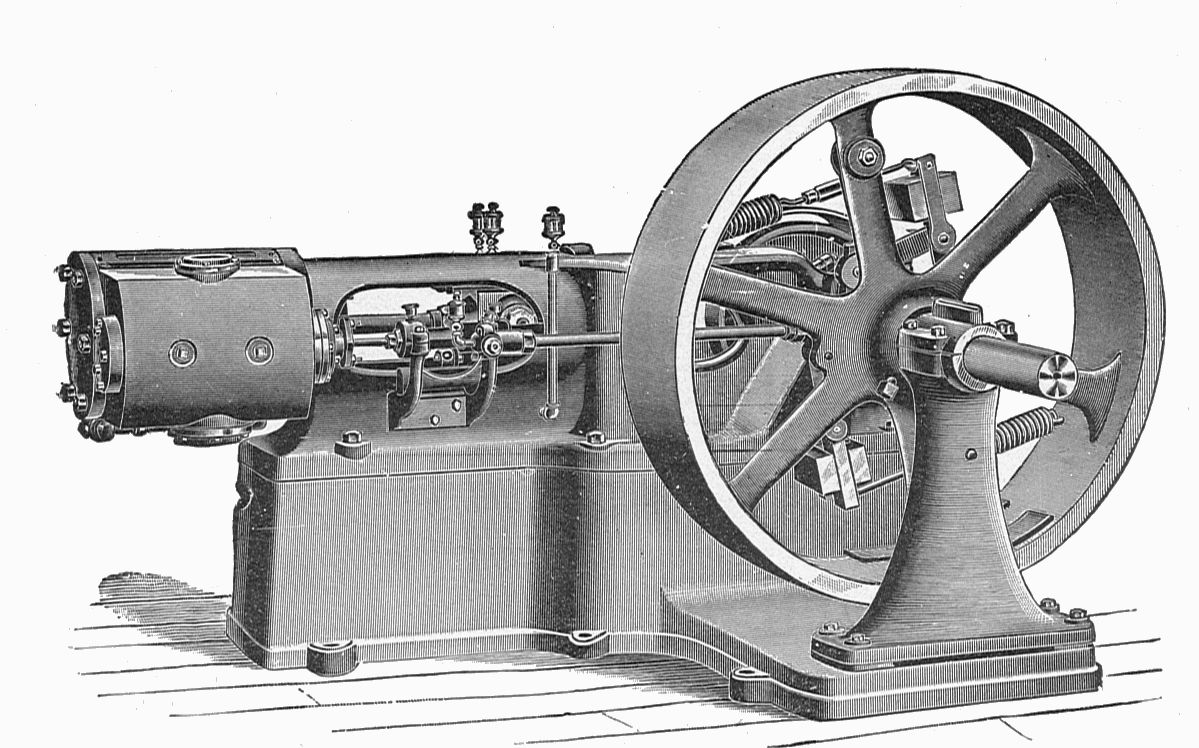
\includegraphics[width=0.5\textwidth]{img/sengine.jpg}};}
\end{frame}

\begin{frame}
 \frametitle{Ptolemy and the almagest}
 \begin{columns}
   \column{0.5\textwidth}\centering
     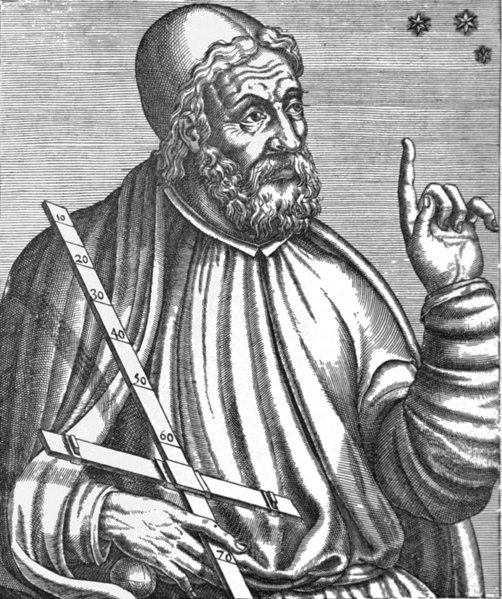
\includegraphics[width=0.8\columnwidth]{img/Ptolemy.png}
   \column{0.5\textwidth}\centering
     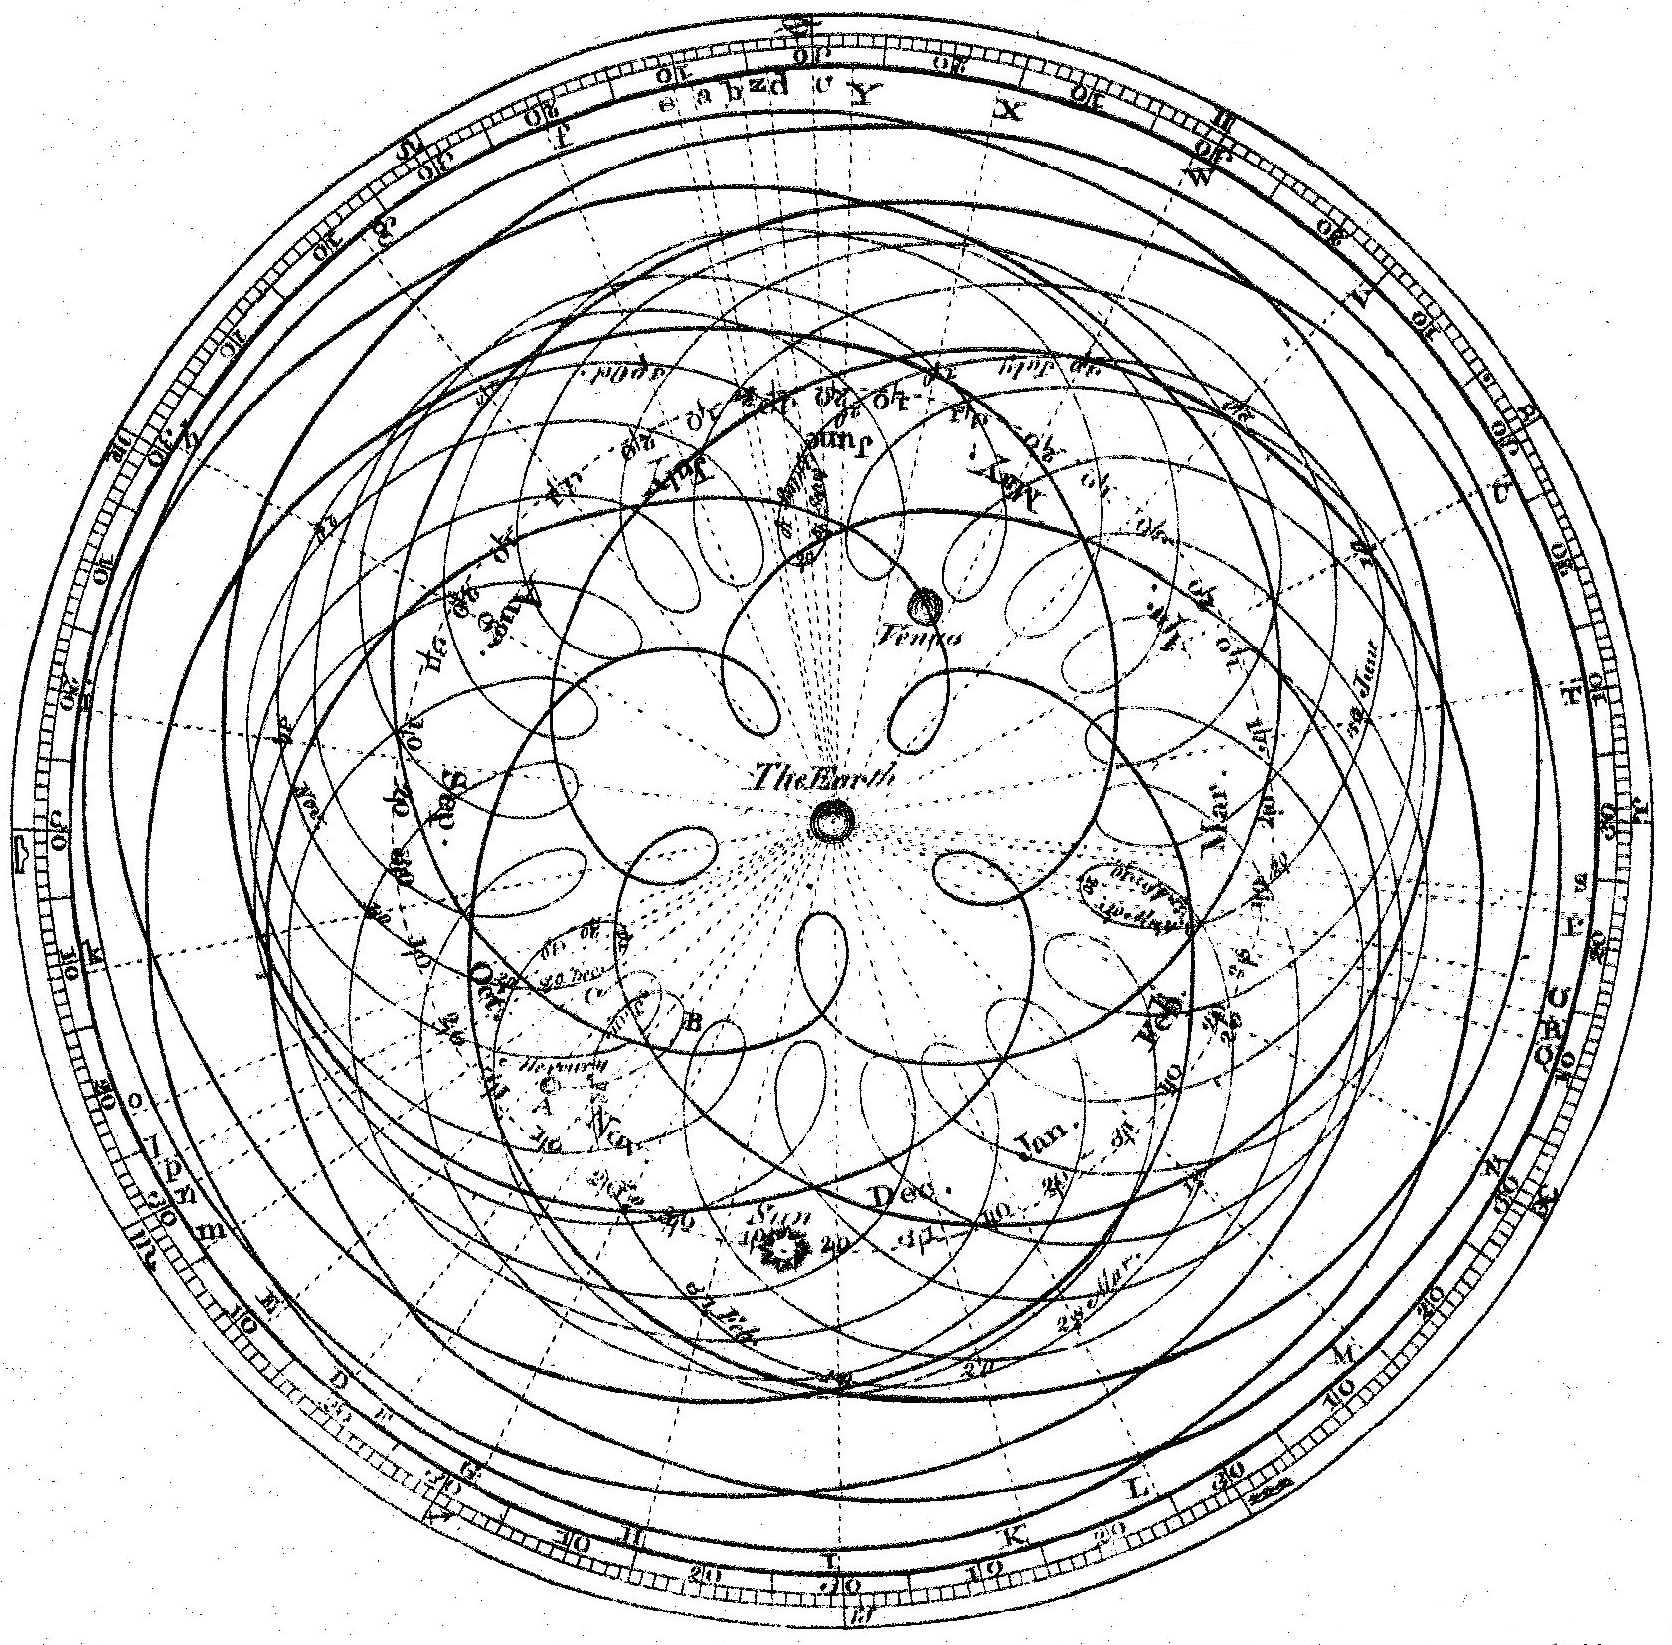
\includegraphics[width=\columnwidth]{img/Cassini_apparent.png}   
 \end{columns} \vspace{1em}
 \tikz{\node[emphblock,text width=\textwidth]{
   ${\sim}150$ AD. Development of numerical approximations to describe the motions of the heavenly bodies with accuracy matching reality sufficiently.};}
\end{frame}

\begin{frame}
 \frametitle{Numerical Methods}
 \begin{itemize}
  \item Numerical analysis is concerned with obtaining approximate solutions to problems while maintaining reasonable bounds of error...
  \item ...because it is often impossible to obtain exact answers ...
  \item Numerical analysis makes use of algorithms to
approximate solutions
 \end{itemize}
\end{frame}

\begin{frame}
 \frametitle{Relevance}
  \begin{itemize}
  \item Important to the world!
  \item E.g. in astronomy, construction, agriculture, architecture, ....
  \item And of course in Engineering!
 \end{itemize}
\end{frame}

\begin{frame}
 \frametitle{...Chemical Engineering...}
  \begin{itemize}
	  \item Description of reactors and separators (dynamic and steady state)
		\item Computational fluid dynamics
		\item Thermodynamic equations of state
		\item Optimizing process performance
		\item Design and synthesis of processes
		\item Regression of data, e.g. isotherms, kinetics, ...
 \end{itemize}
\end{frame}

\section{About this course}
\begin{frame}
 \frametitle{Course Schedule}
 \begin{tabular}{ccll}
 \hline
 Lecture & Date & Topic & Teacher \\ 
 \hline
 1 & 13/11/2017 & Programming and algorithms (1) & IR \\ 
 2 & 16/11/2017 & Programming and algorithms (2) & IR \\ 
 3 & 20/11/2017 & Numerical errors & IR\\ 
 4 & 23/11/2017 & No lecture & \\ 
 5 & 27/11/2017 & Linear eqns: direct methods  & IR\\ 
 6 & 30/11/2017 & Linear eqns: iterative methods & IR\\ 
 7 & 04/12/2017 & Non-linear equations & MSA\\ 
 8 & 07/12/2017 & Interpolation + integration & IR\\ 
 9 & 11/12/2017 & ODEs (1) & MSA\\ 
 10 & 14/12/2017 & ODEs (2) MSA & \\
 11 & 18/12/2017 & PDEs (1) & MSA\\ 
 12 & 21/12/2017 & No lecture & \\ 
 13 & 08/01/2018 & No lecture &  \\ 
 14 & 11/01/2018 & Regression and optimization& IR\\ 
 \hline
 \end{tabular} 
\end{frame}

\begin{frame}
 \frametitle{Course Objectives}
 \begin{itemize}
  \item Gain experience with programming basics and algorithm design
  \item Acquire knowledge of and experience with different techniques for the numerical solution of systems of linear and non-linear algebraic and differential equations, as well as data analysis and optimization.
  \item Being able to solve various numerical problems using Matlab or Excel. 
 \end{itemize}
\end{frame}

\begin{frame}
 \frametitle{Prerequisites}
  The following subjects should give you enough hold-on to follow this course comfortably:
 \begin{itemize}
   \item Calculus A and B
   \item Linear Algebra
   \item Some basic MATLAB experience
     \begin{itemize}
       \item We will shortly cover some aspects on MATLAB programming in the first lectures. Detailed documents and courses are provided on Canvas, for your own reference.
     \end{itemize}
   \item Laptop with Matlab and Excel installed
 \end{itemize}
\end{frame}

\begin{frame}
 \frametitle{Course Materials}
 \begin{itemize}
  \item Lecture slides
  \item MATLAB scripts
  \item Additional articles
  \item There are some useful books:
  \begin{itemize}
    \item Numerical recipes, W.H. Press et al.
    \item Numerical methods for chemical engineering, K.J. Beers
    \item Numerical methods for chemical engineers, A. Constantinides
    \item Essential matlab-for engineers ,B.D. Hahn
    \item Introduction to Numerical Methods and Matlab Programming for Engineers, T. Young and M.J. Mohlenkamp
  \end{itemize}
 \end{itemize}
  \tikz{\node[emphblock,text width=\textwidth]{
    Look on Canvas for the slides, exercises, scripts, assignments and additional documentation on MATLAB.
   };}
\end{frame}

\section{Assessments}
\begin{frame}
 \frametitle{Assessment}
 \begin{block}{5 assignments}
  \begin{itemize}
    \item Each 20\% of the final result
    \item Done in groups of 2 persons
    \begin{itemize}
      \item Form groups via Canvas
      \item Make sure that you have similar intentions!
    \end{itemize}
    \item Short report (template provided, Canvas)
    % \item Resit: 1 assignment + oral exam can be re-done 
  \end{itemize}   
 \end{block}
 \pause
 \begin{block}{About the 5th assignment}
  \begin{itemize}
    \item Short assignment + oral exam (in groups)
    \item Oral exam covers \emph{all assignments and topics}
    \item Individual knowledge is assessed
    \item Grade needs to be at least a 5.0
  \end{itemize}   
 \end{block}
\end{frame} 
\begin{frame}
 \frametitle{Assignment grading}
 We will use rubrics to grade your reports. The following categories will be looked at. \pause
    \begin{itemize}[<+->]
    	\item Use of numerical methods: e.g. built-in solvers vs. show implementation numerical methods
    	\item Analysis of results: just the number is provided vs. high detail analysis and interpretation
    	\item Programming skills: unstructured code, difficult to change vs. readable code with comments and UI
    	\item Visualisation: unreadable graphs with no axes labels or legend vs. publication quality graphs, consistency between datasets
    \end{itemize} 
    \vspace*{2em} \pause
  \tikz{\node[emphblock,text width=\textwidth]{
    The first assignment will be graded via peer-review.};}
\end{frame}
%
%\begin{frame}
% \frametitle{Report structure}
% We want the report to be to the point, describing your approach in solving the numerical problems and giving the results.
% \begin{enumerate}
%   \item Introduction: A few lines in your own words on the goal of the assignment. Don't copy/paste the assignment, we know what it says.
%   \item Results: Provide the results on the question(s) on the assignment. Explain your choices, observations. Make clear graphs (axis labels, readable font). Provide code snippets when you want to illustrate certain nifty tricks, but whole scripts should go in the appendix. Feel free to explore beyond the boundaries of the assignment.
%   \item Discussion and Conclusion: A few lines! Did you achieve your goals, what have you learned?
%   \item Appendix: Provide the scripts and possibly figures that did not make it into the report itself.
% \end{enumerate}
%\end{frame}

%
\begin{frame}
 \frametitle{Assignment handout and deadlines}
     Hand-in your assignments via Canvas
    \begin{itemize}
      \item Deadlines are given on Canvas as well
      \item Deliver the report in PDF format
      \item Send along the scripts + necessities in a .zip
    \end{itemize}
    \tikz{\node[emphblock,text width=\textwidth]{
      When delivering your final assignment, suggest a timeslot for the oral exam (e.g. via Canvas/assignment comment section or as Canvas message).
    };}
\end{frame}
% 
% \begin{frame}
%  \setbeamercolor{alerted text}{fg=tuered}
%  \frametitle{Assignment handout and deadlines}
%  \begin{tabular}{p{0.1\textwidth}ccp{0.4\textwidth}}
%  \hline
%  Assign\-ment & Provided & Deadline & Topic \\ 
%  \hline
%   1 & 9/11/2015 & 23/11/2015 & Programming and algorithms, numerical errors \\ 
%  2 & 19/11/2015 & \alert{07/12/2015} & Linear and non-linear equations  \\ 
%  3 & \alert{03/11/2015} & \alert{17/12/2015} & ODEs, integration and interpolation \\
%  4 & 10/12/2015 & 04/01/2016 & PDEs \\ 
%  5 & 04/01/2015 & 17/01/2016 & Regression and optimization \\ 
%  \hline
%  \end{tabular} 
% \end{frame}

\section{Finally...}
\begin{frame}
 \frametitle{Contact information}
 \begin{block}{Ivo Roghair}
  \begin{itemize}
%    \item Contact via Canvas is preferred!
   \item E-mail: \href{mailto:i.roghair@tue.nl}{i.roghair@tue.nl}
   \item Office: STW 0.37
   \end{itemize} 
 \end{block}
 \vspace{1em}
  \begin{block}{Martin van Sint Annaland}
  \begin{itemize}
   \item E-mail: \href{mailto:m.v.sintannaland@tue.nl}{m.v.sintannaland@tue.nl}
   \item Office: STW 0.39 
   \end{itemize} 
 \end{block}
 \begin{block}{Milan Mihajlovic and Alessandro Battistella}
    For help with the exercises, Milan and Alessandro (STO 1.28) will help out during the lectures.\\
%     Ramon: \href{mailto:r.j.w.voncken@tue.nl}{r.j.w.voncken@tue.nl}\\
%     Alessandro: \href{mailto:a.battistella@tue.nl}{a.battistella@tue.nl}
  \end{block}
\end{frame}

\begin{frame}
 \frametitle{Some last remarks}
  \begin{itemize}
   \item Tell us if something is not clear.
   \item We try to make the lectures interactive, working on examples and creating scripts as we go. It is advised that you work along with us to get the most out of this course!
   \item The exercises are meant to provide a jump start towards the assignments.
   \item We will always answer questions on the exercises. We may didactically answer questions on the assignments.
   \item During the lectures/tutorials we first and foremost work on the exercises. If they are done, you can work on the assignment if you want.
   \end{itemize} 
\end{frame}

\begin{frame}
 \frametitle{Some Acknowledgements}
 \centering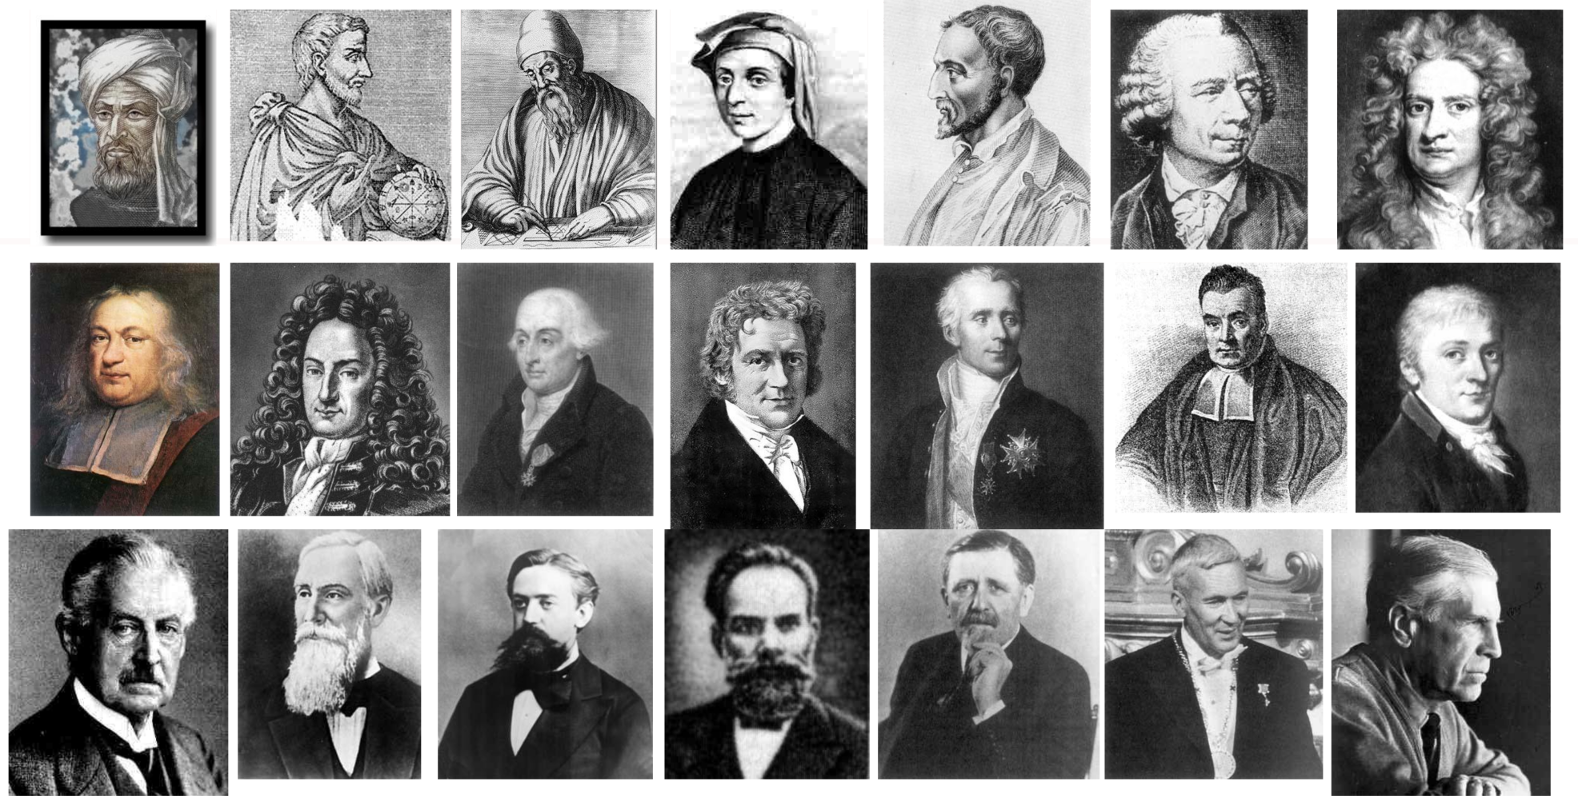
\includegraphics[width=\textwidth]{img/ack.png}
\end{frame}

\begin{frame}
 \frametitle{Some Real Acknowledgements}
 \begin{itemize}
  \item To Roel Verstappen of Groningen University
  \item To Johan Hult of Cambridge University
  \item To Edwin Zondervan, now at Universit\"at Bremen
 \end{itemize}
\end{frame}
\end{document}


% References
% http://ocw.mit.edu/courses/electrical-engineering-and-computer-science/6-00sc-introduction-to-computer-science-and-programming-spring-2011/unit-1/lecture-1-introduction-to-6.00/
% http://www.greenteapress.com/thinkpython/html/thinkpython002.html
% https://www.youtube.com/channel/UCLMQ21H2ad95faYG3yGCwYA
%http://stackoverflow.com/questions/4227145/in-matlab-are-variables-really-double-precision-by-default
%http://www.exploringbinary.com/why-0-point-1-does-not-exist-in-floating-point/

